\documentclass{article}

\title{Pascal Scanner - Software Design Document}
\date{2016-12-6}
\author{Allen Burgett}

\usepackage{pdfpages}

\begin{document}

\pagenumbering{gobble}
\maketitle
\pagebreak

\pagenumbering{arabic}

\section{Summary}
This program can scan a document for Pascal type tokens and return them to the user.

\section{Structure}
The program relies primarily on JFlex, a Java program that builds a state machine to process a grammar. The JFlex spec file contains all the criteria for what constitutes as a Pascal token. The JFlex spec generates Java code, based on the defined state machine. This Java can be compiled and added to an existing Java Program.

\subsection{MyScanner.JFlex}
This file defines the parameters of a state machine. The generated state machine is used to identify Pascal Tokens.

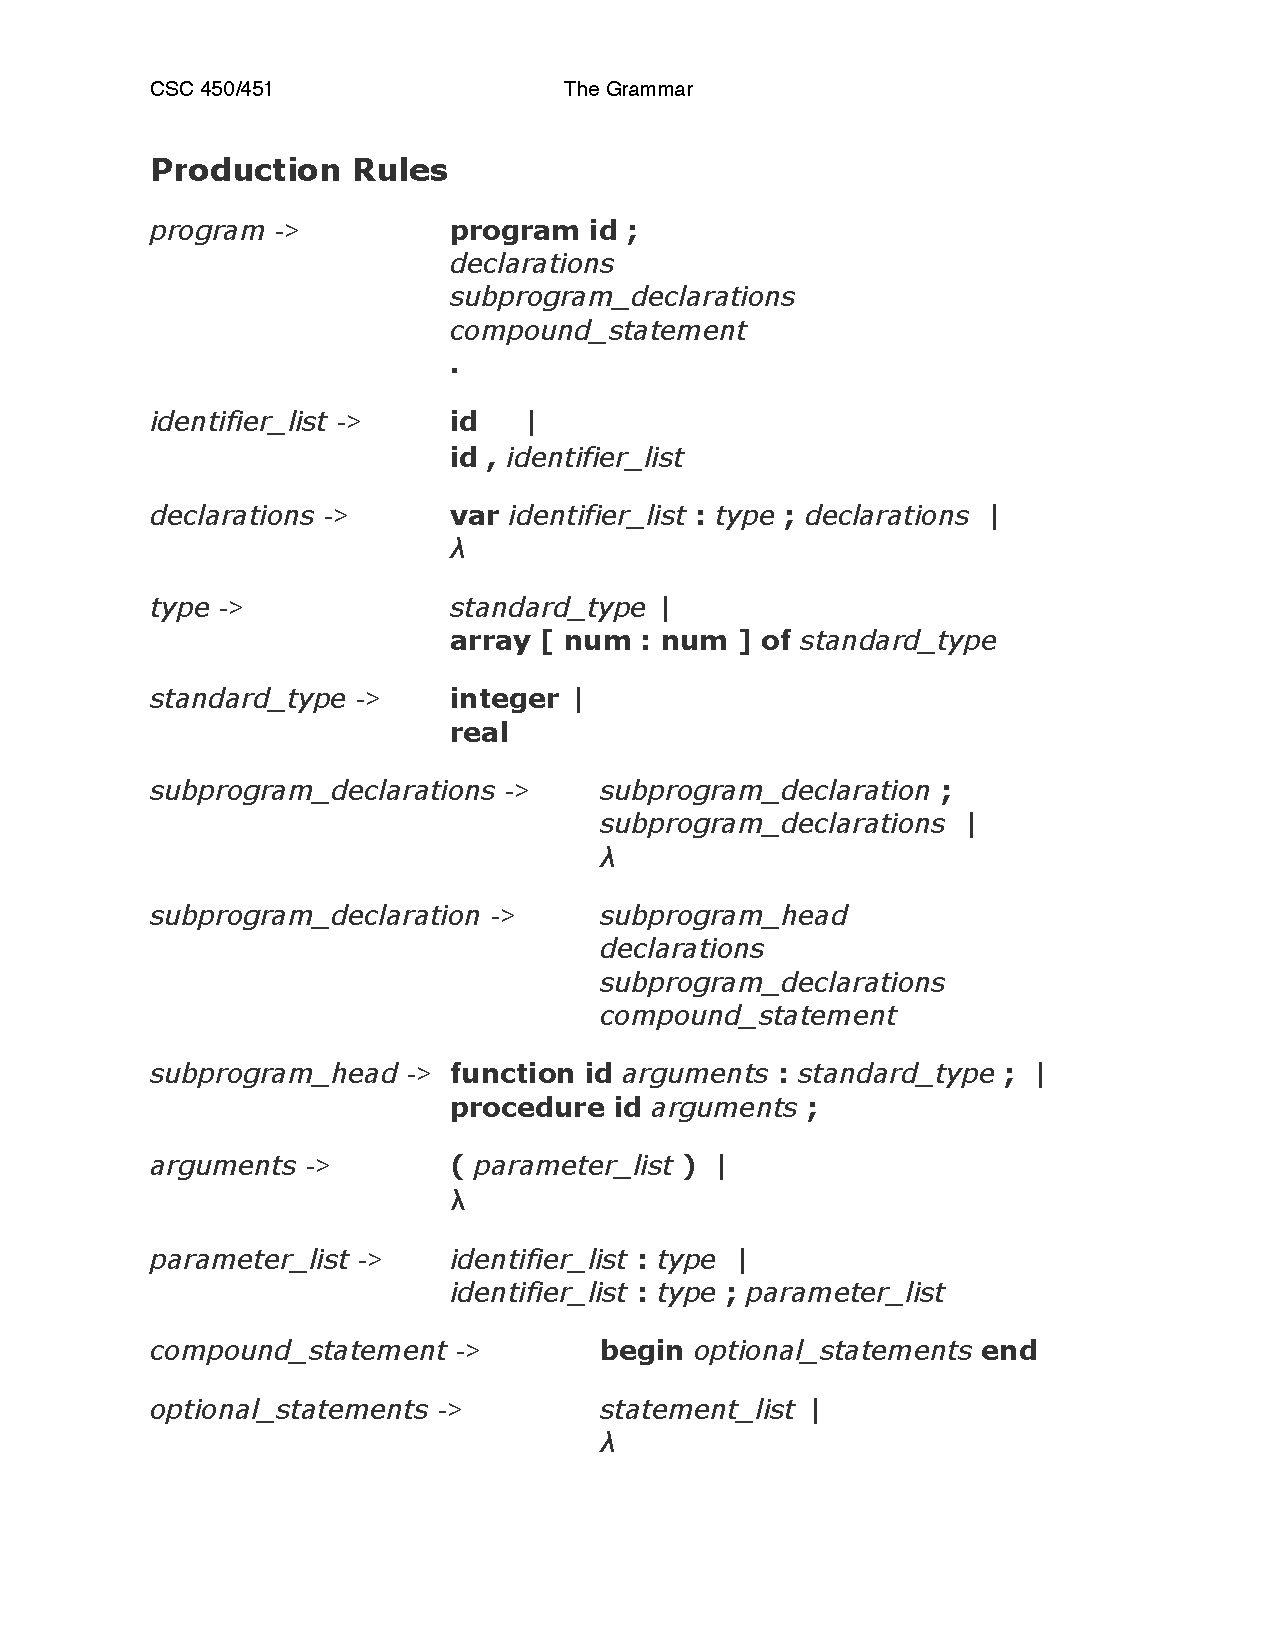
\includepdf[pages={-}]{Grammar.pdf}

\end{document}

